\section{全景漫游与人的心理特征}

\subsection{知觉}
人们通过感官得到了外部世界的信息,这些信息经过头脑的加工(综合与解释),产生了对事物整体的认识,就是知觉(perception)。\endnote{彭, 聃龄. 普通心理学[M]. 北京师范大学出版社, 2004.}知觉按照是由人体感官或是人脑后天习得的事物特性可分为两类:前文所列举的视觉、听觉和平衡感觉等都属于第一类,而下文所涉及到的空间知觉和时间知觉则属于后天根据既往经验认知得到的第二类感觉,其特征是受环境影响大,易被外在因素所影响。在进行全景漫游活动中,后一类知觉更易受场景画面、环境声响甚至温度湿度等变化而发生改变。

\subsubsection{空间知觉}
空间知觉是指人对物体、环境等单体或多个在空间关系上的认知。其包含形状、大小、距离、方位等,在人辨别与周围环境的相互关系中起重要作用。

人可以分辨距离的能力主要来源于双眼视差和眼球变焦。双眼视差是指物体在人的左眼及右眼中分别投射的影像是不同的,根据成像距离的不同将使人产生与物体间的距离感,这也是包括 3D 眼镜在内的所有模拟立体成像技术的基本原理,如图\ref{fig:eyes}。

\begin{figure}[htp]
\centering
\fbox{
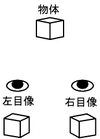
\includegraphics[width=.2\textwidth]{eyes}
}
\caption{双眼成象}
\label{fig:eyes}
\end{figure}

眼球变焦是指在人在观察一定距离外的物体时,需要调整睫状肌带动眼中的晶状体来进行对焦。而当晶状体发生改变时,眼球中接收到的光线就是不同距离和角度的光线了,称为眼球的“适应性调节”。人眼同时需要转动一定角度以适应这种对焦引起的改变,这种调节过程称为“视觉辐辏”。上述两者一般是成双成对地出现,这是一种正常的生理反应,如图\ref{fig:binocular_disparity}。但当配戴上全景眼镜时,人眼在注视不同物体时仍会产生上述两种反应,但因为全景图像没有景深,即所有场景内物体的焦距都是相差无几的,这时便造成了视觉辐辏和适应性调节后无法准确对焦物体,造成了视觉冲突。这种冲突称为“视觉辐辏调节冲突“,将会在一定时间后带来晕眩不适感\endnote{李书印,万明习,李新肖,刘凯文. 虚拟环境中的视觉感知[J]. 中国图象图形学报,2000,(11):28-32.}。

\begin{figure}[htp]
\centering
\fbox{
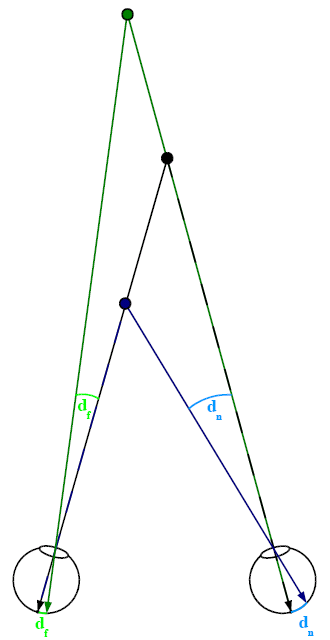
\includegraphics[width=.2\textwidth]{binocular_disparity}
}
\caption{视觉辐辏和适应性调节}
\label{fig:binocular_disparity}
\end{figure}

目前能够完美解决这种冲突的方式是还原出物体的真实景深信息\endnote{刘红民. 立体深度图像的形成和立体3D图像的视觉舒适增强[D].西安电子科技大学,2014.},使得双眼在屏幕上不同焦距时可以看到成不同像的物体。但现阶段该技术仍处在研究状态,当前可以缓解这种全景图像没有景深的方式是尽量在不影响画面完整度的情况下缩小场景内物体间景深的差距,以使眼球的视觉辐辏与适应性调节产生的偏差尽可能小。

\subsubsection{时间知觉}
时间流逝的速率在正常环境下几乎是不变的,但人对时间的概念却因很多因素而发生改变。人对时间的判断依赖于人脑对事物事件的发生次序和连贯性的综合评价,也与人当前的生理状态有关。

在全景漫游中,场景中发生的所有事件都一一呈现在眼前,人脑长时间暴露在大量信息的处理过程中,会觉得时间过的很快(类似于沉迷于网络游戏的青少年永远也不觉得自己玩游戏时间过长)。而且全景场景中事物的一般运动在距人眼非常近的情况下变得非常明显,更是进一步加剧了人对时间流逝的估计\endnote{凤四海,黄希庭. 时间知觉理论和实验范型[J]. 心理科学,2004,(05):1157-1160.
}。

单纯从体验角度来观察用户在使用全景漫游设备时的时间知觉意义并不明显,但结合现有关于使用全景漫游设备体验后造成不适的例子可以看出,大部分体验者在摘下眼镜后的数分钟甚至数十分钟内均有一定的不适应感,表现为对外界环境的陌生感和行为上的迟钝感。

若要在全景漫游中保持人正常的时间知觉能力,应当适当降低场景中事物的数量和并发量,以减少人脑所需处理的信息量,使人能处于一种比较平和的体验过程。这样既可以缓解人的紧张情绪以使人可以更长时间且不疲劳地进行全景漫游体验,又能让人在场景中注意到更多细节之处,提升体验质量\endnote{毕翠华. 工作记忆的保持影响时间知觉的认知与神经机制[D].西南大学,2014.}。

\subsection{意识}
意识可以被认为是个体对客体的一系列相关的知觉,是一种心理状态,对信息的觉察和感知,甚至还具有能动性和调节作用。

\subsubsection{选择性注意}
选择性注意是指在多种刺激中选择一种进行注意,同时忽略或减少注意其他的刺激。现有研究大多是经实验分析推测选择性注意的过程,比较著名的理论有“过滤器理论”、“衰减理论”、“后期选择理论”和“多阶段选择理论”。而上述理论都是假设注意是一个容量有限的通道,则注意的过程像是一把筛子,筛选出那些需要感觉器官反应的刺激。认知资源理论认为人的认知系统对刺激的识别需要占用认知资源,越复杂的刺激需要越多的认知资源;为了处理更多“被认为是重要的刺激”,人脑需要将有限的认知资源向更重要的刺激分配,因而忽视掉那些不是很重要的刺激。双加工理论认为人类的认知加工有两种:自动化加工和受意识控制的加工,两者并行运作,各有各自的认知过程,且可以互相转换、影响。

综合上述理论可知,人对刺激的注意程度是不一样的,人会对那些“自己觉得重要”或是“超过一般强度”的刺激进行注意\endnote{张明,张阳. 工作记忆与选择性注意的交互关系[J]. 心理科学进展,2007,(01):8-15.}。在全景漫游中,交互设计应注意刺激的强度和持续时间,不宜出现过于突然的刺激,以免令用户产生过大的注意,而忽视正常的安全防范或作出过当的反应(如全景漫游体验过山车或造成没有准备的体验者过于激烈的心跳反应甚至危害健康)。同时也不宜使人长期处在过大的刺激中,有可能提高了人注意的反应阈限以致在体验过程后产生认知失调的现象。

\subsubsection{持续性注意与意识动摇}
持续性注意是指在一段时间内保持注意某事物的现象。人为了满足生产工作学习的需要,必须有或长或短的注意持续时间。而与之对应的是注意动摇,即短时间内注意力发生变化。

需要明确的是,注意动摇并不总是一种不好的现象,因为人持续聚精会神的时间越长越容易发生注意动摇,所以日常活动或是游戏中常见有特意设置分散注意力的动作以调整人的注意力。比如图\ref{fig:magnet}是某款手机跑酷游戏,通过设置特殊道具来吸引玩家注意力,以避免无意识的注意动摇。

\begin{figure}[htp]
\centering
\fbox{

\includegraphics[width=.5\textwidth]{magnet}
}
\caption{某手机游戏截图}
\label{fig:magnet}
\end{figure}

\subsection{认知}
人类认知是非常复杂的过程,以下只列举了具有代表性的几种心理过程。认知在日常活动中起到了重要的作用,可以说没有认知过程人就无法进行任何需要动脑才能完成的工作和任务。

\subsubsection{记忆}
记忆是指头脑中积累和保存个体经验的心理过程,运用信息加工的术语讲,就是人脑对外界输入的信息进行编码、存储和提取的过程。记忆按信息保持时间的长短可分为感觉记忆(即瞬时记忆)、短时记忆和长时记忆。在全景漫游中,这三种记忆都非常重要\endnote{刘兆敏,郭春彦. 工作记忆和长时记忆共享信息表征的ERP证据[J]. 心理学报,2013,(03):276-284.}。

感觉记忆只有 0.25
~2 秒,是屏幕图像组合成人脑中运动画面的关键因素。短时记忆则是漫游过程的直接材料,比如上文提到的射箭游戏,即是利用人短时建立起来的关于“手柄 = 弓和箭”的记忆,使得用户在一次成功尝试后便可利用该记忆完成后续数十次操作以完成游戏。而短时记忆在脱离记忆场景后会进入长时记忆中,但不会一直被唤起。因此使用者在结束全景漫游后不会继续将其他手柄也认作为是游戏中的“弓和箭”进行操作,但在下一次游戏时使用者便可不经提示就能直接上手操作手柄完成游戏中“拉开弓并射出箭”的操作,这时短时记忆就变成了长时记忆。

\subsubsection{思维}
思维是人对外通过多种方式表现出的对客观事物的认识,是认识的高级形式。如果以相同输入而言,人对信息的加工过程就体现了思维的不同。思维的形式和理论有很多,在此只列举一个与本文贴近的假设以做参考。

人脑中基本的认知单位是概念,是人对客观事物的本质特征的认识。概念又可分为自然概念和人工概念两类,如何形成人工概念的途径也有很多假说。有布鲁纳等人提出的假设检验(hypothesis test model)认为,概念形成的过程是不断提出假设、验证假设的过程。人不会无端形成一种概念,其在不被告知正确概念的时候可以通过试错的方式来检验自身的假设是否正确,如果得到正确的反馈则验证了假设,反之则催使进行更多的假设。而成功的假设可能形成记忆,将认知保留在长时记忆中以供后续使用\endnote{焦璨,张敏强. 迷失的边界:心理学虚无假设检验方法探究[J]. 中国社会科学,2014,(02):148-163+207.}。

较为典型的案例是,现在各种电子产品的说明书越来越薄,甚至于全部功能都留给用户自己来发掘。当用户在第一次使用触屏手机浏览图片时,发现没有熟悉的滚轮缩放图片大小的功能,会尝试性地通过各种方式来放大图片,而在某一次尝试中会发现“双指缩放”可以达到这种效果从而成功验证了假设,完成了概念的形成,如图。此后,即使是到了其他设备上,用户也能够利用这一概念顺利地完成类似操作。

\begin{figure}[htp]
\centering
\fbox{
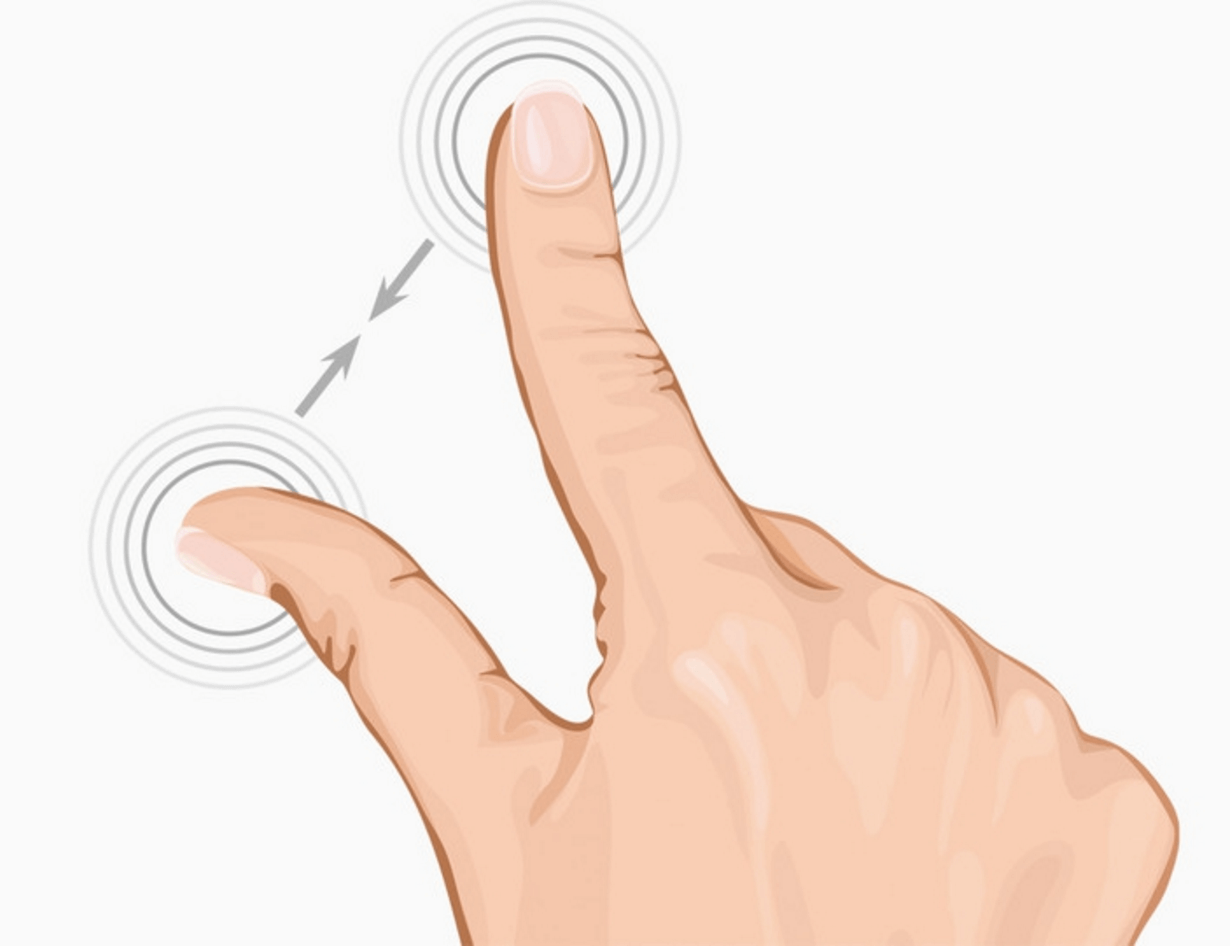
\includegraphics[width=.5\textwidth]{stretch}
}
\caption{双指缩放}
\label{fig:stretch}
\end{figure}

\subsubsection{动机}
动机是由目标或对象引导、激发和维持个体活动的一种内在心理过程或内部动力。动机能够激发行为,且能引导行为的发展。马斯洛的需求层次理论认为,人的生理需求处于金字塔的末端,而自我实现和尊重的需要处于金字塔的顶端。人天生是一类勇于探索的生物,从海洋到陆地,从森林到草原,从石器到电气,人类进步最大的动机就是探索未知的世界。一个人若想自我实现所能达到的最高成就,便是在人类未知的领域去迈出自己的一步。古往今来,哥伦布、麦哲伦、阿姆斯特朗等都是代表人类迈出了探索世界的脚步,探索的精神已经深深植入人类的心底,戴上眼镜,进入全景漫游的世界,对于个体而言即是相当于自我探索的一大步,这也就是全景漫游技术所带给体验者最好的礼物。
